\documentclass{standalone}

\usepackage{tikz}
\usetikzlibrary{shapes.geometric}
\begin{document}
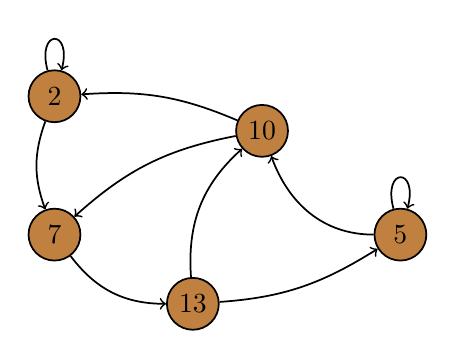
\begin{tikzpicture}
[every node/.style={inner sep=0pt}]
\node (2) [circle, minimum size=18.75pt, fill=brown, line width=0.625pt, draw=black] at (37.5pt, -25.0pt) {\textcolor{black}{2}};
\node (7) [circle, minimum size=18.75pt, fill=brown, line width=0.625pt, draw=black] at (37.5pt, -75.0pt) {\textcolor{black}{7}};
\node (13) [circle, minimum size=18.75pt, fill=brown, line width=0.625pt, draw=black] at (87.5pt, -100.0pt) {\textcolor{black}{13}};
\node (5) [circle, minimum size=18.75pt, fill=brown, line width=0.625pt, draw=black] at (162.5pt, -75.0pt) {\textcolor{black}{5}};
\node (10) [circle, minimum size=18.75pt, fill=brown, line width=0.625pt, draw=black] at (112.5pt, -37.5pt) {\textcolor{black}{10}};
\draw [line width=0.625, ->, color=black] (10) to  [in=4, out=157] (2);
\draw [line width=0.625, ->, color=black, loop above] (2) to (2);
\draw [line width=0.625, ->, color=black, loop above] (5) to (5);
\draw [line width=0.625, ->, color=black] (2) to  [in=110, out=250] (7);
\draw [line width=0.625, ->, color=black] (7) to  [in=180, out=307] (13);
\draw [line width=0.625, ->, color=black] (13) to  [in=222, out=94] (10);
\draw [line width=0.625, ->, color=black] (10) to  [in=42, out=191] (7);
\draw [line width=0.625, ->, color=black] (13) to  [in=212, out=4] (5);
\draw [line width=0.625, ->, color=black] (5) to  [in=290, out=180] (10);
\end{tikzpicture}
\end{document}
